\documentclass[12pt]{article}
%\usepackage{tkiz}

\usepackage[utf8]{inputenc}
\usepackage[french]{babel}
\usepackage{amsmath,amsthm,amsfonts,amssymb}
\usepackage{lmodern}
\usepackage[top=2.4cm,bottom=2.4cm,left=2cm,right=2cm]{geometry}
\usepackage{hyperref}
\usepackage{multicol}
\usepackage{enumitem}
\usepackage{listings}
\usepackage[dvipsnames]{xcolor}
\usepackage{tikz}

%\date{}
\title{{\bf  Génie logiciel} \\
	Notes du cours de 14/10 , partie 2 \\
	{\small L3 Informatique appliquée 2022-2023} \\
	{\it \small MABROUK Fayez}}
\begin{document}
	\maketitle
\newpage
\section{Diagramme des cas d'utilisation}
\subsection{Cas d'utilisation}
\begin{itemize}
	\item [*] Définition : Un cas d'utilisation est la spécification d'un ensemble d'actions exécutées par un système,qui produit un résultat observable qui a, en général, de la valeur pour un ou plusieurs ou plusieurs acteurs ou autres parties prenantes du système. (OMG UML Superstructure 2.0).
	\item [*] Définition : un acteur est le rôle d'un utilisateur externe lors de l'interaction avec le
	système.
	\item [*] Vue externe (point de vue des acteurs) du système.
	\item [*] Capture des exigences fonctionnelles.
	\item [*] Un cas d'utilisation décrit les actions et les interactions avec le système pour une
	exigence fonctionnelle.
	\item [*] Support pour toutes les autres étapes du développement logiciel.
\end{itemize}
\subsection{L'acteur}
\begin{itemize}
	\item [*] Externe au système.
	\item [*] Interagit directement avec le système.
	\item [*] A un rôle (en général, indiqué par son nom).
	
\end{itemize}
\subsection{Diagrammes de cas d'utilisation}
\begin{itemize}
	\item [*] Définition : Un diagramme de cas d'utilisation montre un ou plusieurs cas d'utilisation, un ou plusieurs
	acteurs, et les relations entre eux.
	

\begin{figure}[!hbtp]
	%\centering
	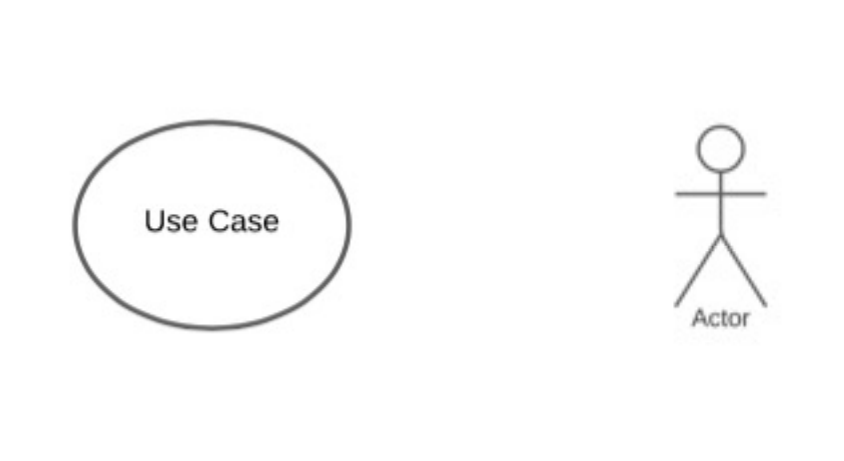
\includegraphics[scale=0.75]{Capture.PNG}
	%\caption{Légende de l'image}
\end{figure}

	\line(1,0){100} 	\flushright{Les acteurs et les cas d'utilisation sont
		liés par une association
		lien.}
\end{itemize}
\subsection{Éléments des diagrammes de cas d'utilisation}
\newpage
\begin{itemize}
	\item [*] Le cas d'utilisation est nommé (le nom doit être descriptif !).
	\item [*] Optionnellement, le système peut être représenté par un rectangle. 
	\begin{figure}[!hbtp]
	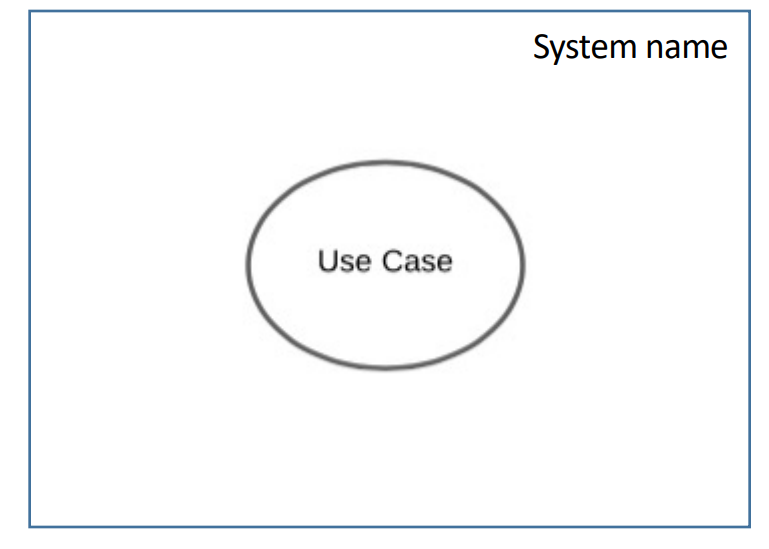
\includegraphics[scale=0.75]{Capture1.PNG}	
	\end{figure}
	\item [*] Un acteur peut être :
	\begin{itemize}
		\item [*] primaire : celui pour lequel l'objectif du cas d'utilisation est essentiel. Le plus souvent, il initiera
		le cas d'utilisation.
		\item [*] secondaire : l'objectif n'est pas essentiel, mais il est tout de même en interaction avec le cas d'utilisation.
	\end{itemize}
\item [*] Convention : les acteurs primaires à gauche et les acteurs secondaires à droite du ou des
cas d'utilisation.
\item [*] Si le système est dessiné, les acteurs sont à l'extérieur.
\item [*] Un lien d'association entre un acteur et un cas d'utilisation indique que l'acteur peut
interagir avec le cas d'utilisation.
\item [*] Une association peut être représentée par :
\begin{itemize}
	\item [*] un lien complet. \line(1,0) {100}
	\item [*] une flèche indiquant qui a initié l'interaction.
\end{itemize}
\item [*] Par conséquent : une association entre un cas d'utilisation et un acteur secondaire est une flèche !\\ 
\\
\begin{tabular}{|r|l|}
	\hline
	Représentation & Cardinalité \\
	\hline
1 & Exactement une fois \\
	N & Exactement n fois  \\
	* & N'importe quel nombre (y compris 0) de fois \\
	0..1 & 0 ou une fois \\
	1..* & Une ou plusieurs fois\\
	M..N & De M à N fois\\
	\hline
\end{tabular}
\\
\item[*] Les associations entre un acteur
et un cas d'utilisation peuvent avoir une
cardinalité.
\item[*] Cardinalité du côté du cas d'utilisation
d'utilisation : combien d'instances du
cas d'utilisation (scénario) l'acteur
l'acteur est lié ?
\item[*] Cardinalité du côté de l'acteur :
combien d'instances de l'acteur
l'acteur sont liées à une instance
du cas d'utilisation ?
\item[*] Possibilité d'utiliser des notes.
\item [*]  Utile pour indiquer
les acteurs primaires/secondaires.
\end{itemize}
\end{document}